\section{Ensemble-Methoden}
\label{sec:dt_ensemble_methods}
Ensemble-Methoden beschreiben wie mehrere Entscheidungsbäume trainiert werden, um eine möglichst hohe Diversität der einzelnen Entscheidungsbäume zu erzielen. Das Ergebnis eines Ensembles
ist die Aggregation der Ergebnisse der einzelnen Entscheidungsbäume \cite{dietterich2002ensemble}.
\newline
\newline
Der Wahlklassifizierer $H(x) = w_1 h_1(x) + ... + w_K h_K(x)$ ist eine Möglichkeit die Einzelergebnisse $\{h_1, ..., h_K\}$ gewichtet mit $\{w_1, ..., w_K\}$ zu aggregieren \cite{dietterich2002ensemble}.
Ein Ergebnis kann auf zwei Arten modelliert sein. Einerseits als eine Funktion $h_i: D^n \mapsto \setR^m$, die einer $n$-dimensionalen Menge $D^n$ jeder der $m$ möglichen Klassen eine Wahrscheinlichkeit
zuweist. Das Ergebnis ist eine Wahrscheinlichkeitsverteilung. Das diskrete Ergebnis der Klassifizierung ist die Klasse mit der höchsten Wahrscheinlichkeit in dem Ergebnis.
Andererseits kann es als eine Funktion $h_i: D^n \mapsto M$ abgebildet werden, die diskret auf eine der möglichen Klassen in $M$ verweist \cite{dymelThesis}. In diesem Fall wird die Klasse ausgewählt, die am
häufigsten unter allen Einzelergebnissen vorkam. In der Praxis wird die Aggregation der Wahrscheinlichkeitsverteilung genutzt \cite{ScikitLearnEnsemble}.
Analog ist $H: D^n \mapsto \setR^m$ oder $H: D^n \mapsto M$ definiert \cite{dietterich2002ensemble}. Für gewöhnlich hat jeder Teilnehmer einer Wahl das gleiche Gewicht.
\newline
\newline
Bagging (\textbf{B}ootstrap \textbf{agg}regat\textbf{ing}) konstruiert Entscheidungswälder, indem es Entscheidungsbäume mit Teilmengen der Trainingsmenge trainiert.
Abbildung \ref{fig:bagging} illustriert die Bagging Methode für $n$ Entscheidungsbaummodelle. Zunächst wird die Trainingsmenge in $n$ Teilmengen aufgeteilt \cite{breiman1996bagging}.
Der Inhalt der Teilmengen wird mit der \glqq Bootstrap sampling\grqq\ Methode bestimmt. Diese zieht aus einer Grundmenge $l$-mal jeweils $k$-Einträge \cite{efron1992bootstrap}.
Mit jeder Teilmenge wird ein Entscheidungsbaum trainiert \cite{breiman1996bagging}. Die Einzelergebnisse werden aggregiert, z. B. mit dem Wahlklassifizierer.
\begin{figure}[h!]
    \centering
    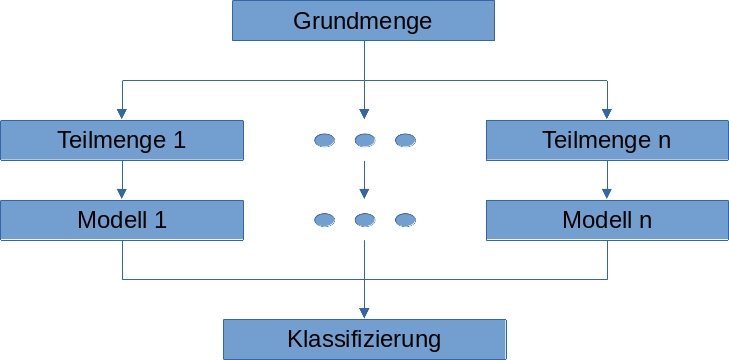
\includegraphics[width=0.6\linewidth]{images/bagging.jpg}
    \caption{Klassifizierungsprozess mit der Bagging-Methode.}
    \label{fig:bagging}
\end{figure}
\newline
\newline
Random Forest erweitert die Bagging-Methode \cite{breiman2001random}. Für jeden Entscheidungsbaum der trainiert werden soll, wird zusätzlich zufällig eine Teilmenge der Feature-Menge ausgewählt.
\newline
\newline
Extremely Randomized Trees (ExtraTrees) verwenden ebenfalls eine Teilmenge der Feature-Menge der Trainingsmenge beim Trainieren der einzelnen Entscheidungsbäume \cite{geurts2006extremely}.
Allerdings wird für jeden Entscheidungsbaum die gesamte Trainingsmenge verwendet. Dies soll den Bias reduzieren. Bei der Konstruktion wird nicht versucht die beste Teilungsregel zu finden,
sondern es werden zufällig Teilungsregeln generiert, aus denen die Beste ausgewählt wird. Dieses Verfahren soll die Varianz reduzieren.
\newline
\newline
Beim Boosting werden nacheinander schwache Lerner auf einer Teilmenge trainiert, die gewichtet aggregiert werden \cite{freund1997decision}. Dadurch entsteht ein starker Lerner.
Abbildung \ref{fig:boosting} illustriert, wie vier schwache Lerner trainiert werden. Jeder Lerner findet eine Funktion der die trainierte Teilmenge unterteilt. Anschließend
werden sie gewichtet aggregiert. Dies konstruiert einen starken Lerner, der die gesamte Trainingsmenge unterteilt. Diese Arbeit verwendet \texttt{AdaBoost} \cite{freund1997decision} von Freund und Schapire.
\begin{figure}[h!]
    \centering
    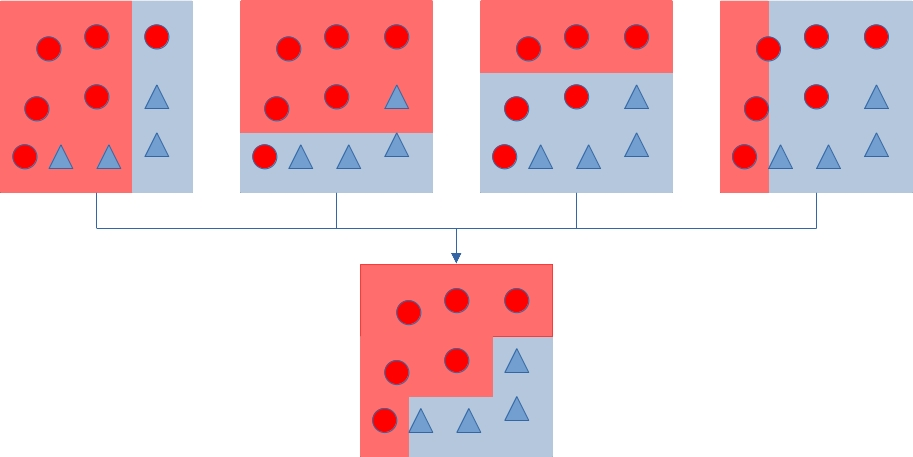
\includegraphics[width=\linewidth]{images/boosting.jpg}
    \caption{Klassifizierungsprozess mit der Boosting-Methode.}
    \label{fig:boosting}
\end{figure}